%Laborationsrapport

\documentclass[a4paper,12pt,fleqn]{article}
\usepackage{fixltx2e}
\usepackage[utf8]{inputenc}
\usepackage{graphicx}
\usepackage{sidecap}
\usepackage{fancyhdr}
\usepackage{amssymb,amsmath}
\usepackage[swedish]{babel}
\usepackage[margin=1.5in]{geometry}
\usepackage{abstract}
\usepackage[parfill]{parskip}
\usepackage{tocloft}
\usepackage{adjustbox}
\usepackage{textcomp}
\usepackage[T1]{fontenc}
\usepackage{listings}
\usepackage{xcolor,colortbl}
\usepackage{hyperref}
\usepackage{perpage} %the perpage packag

%----------------------------------------------------------------
%C-kod formatering

\definecolor{listinggray}{gray}{0.9}
\definecolor{lbcolor}{rgb}{0.9,0.9,0.9}
\lstset{
backgroundcolor=\color{lbcolor},
    tabsize=4,    
%   rulecolor=,
    language=[GNU]C++,
        basicstyle=\scriptsize,
        upquote=true,
        aboveskip={1.5\baselineskip},
        columns=fixed,
        showstringspaces=false,
        extendedchars=false,
        breaklines=true,
        prebreak = \raisebox{0ex}[0ex][0ex]{\ensuremath{\hookleftarrow}},
        frame=single,
        numbers=left,
        showtabs=false,
        showspaces=false,
        showstringspaces=false,
        identifierstyle=\ttfamily,
        keywordstyle=\color[rgb]{0,0,1},
        commentstyle=\color[rgb]{0.026,0.112,0.095},
        stringstyle=\color[rgb]{0.627,0.126,0.941},
        numberstyle=\color[rgb]{0.205, 0.142, 0.73},
%        \lstdefinestyle{C++}{language=C++,style=numbers}’.
}
\lstset{
    backgroundcolor=\color{lbcolor},
    tabsize=4,
  language=C++,
  captionpos=b,
  tabsize=3,
  frame=lines,
  numbers=left,
  numberstyle=\tiny,
  numbersep=5pt,
  breaklines=true,
  showstringspaces=false,
  basicstyle=\footnotesize,
%  identifierstyle=\color{magenta},
  keywordstyle=\color[rgb]{0,0,1},
  commentstyle=\color{Darkgreen},
  stringstyle=\color{red}
  }
  %-----------------------------------------------------------------
  %marginaler

  \renewcommand{\abstractnamefont}{\normalfont\normalsize\bfseries}
  \renewcommand{\abstracttextfont}{\normalfont\small}
  \renewcommand{\headrulewidth}{0pt}
  \renewcommand{\cftsecleader}{\cftdotfill{\cftdotsep}} 
  \setlength{\absleftindent}{0pt}
  \setlength{\absrightindent}{0pt}
  \setlength{\headheight}{15pt}

  \addtolength{\oddsidemargin}{-.5in}
  	\addtolength{\evensidemargin}{-.5in}
  	\addtolength{\textwidth}{1in}


  %-----------------------------------------------------------------
  %header and footer

  \pagestyle{fancy}
  \lhead{
  	\begin{picture}(0,0)
  		\put(5,0){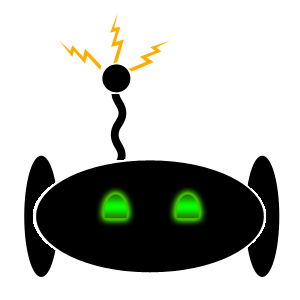
\includegraphics{logotyp.png}}
  	\end{picture}}
	
  \fancyhead[C]{\small{Mapmaster2001}}
  \fancyhead[R]{\small \today}
  \fancyfoot[L]{\small{TSEA56 \\ LIPS Kappa}}
  \fancyfoot[C]{\small{\thepage}}
  \fancyfoot[R]{\small{Projektgrupp 8 \\ mapmaster2001@cyd.liu.se}}

  %-----------------------------------------------------------------

%-------------------------------------------------------------------
%Första sidan
\begin{document}
	\pagestyle{fancy}
	\pagenumbering{gobble}
	\vspace*{\fill}
		\begingroup
			\begin{center}
				\huge{\textbf{Trådlös kommunikation}}
				\\
				\vspace{10pt}
				\normalsize
				Niklas Ericson och Jens Edhammer
				\\
				Kandidatprojekt Y - Grupp 8 - VT2014
				\\
				Version 1.0
				\end{center}
		\endgroup
	\vspace*{\fill}
	
	\begin{center} %Börjar centrering 
		Status
		\\
		\vspace{3pt} %Whitespace 3 pts
	    \begin{tabular}{| p{3cm} | p{3cm} | p{3cm} |} %tabell, 4 horizontella |, 3 cm emellan dem.
	    \hline %översta horizontella linjen.
	    Granskad & - & \today \\ \hline % & -tecken för att "gå till nästa ruta" 
		Godkänd & - & - \\ \hline % avslutas med \\ och \hline.

	    \end{tabular}
	\end{center}
	\vspace{2cm}
	\newpage
%-----------------------------------------------------------------
%Projektidentitet
	
	\vspace*{\fill}
		\begingroup
			\begin{center}
				\LARGE{\textbf{PROJEKTIDENTITET}}
				\\
				\footnotesize
				Grupp 8, 2014/VT, MapMaster2001
				\\
				Tekniska högskolan vid Linköpings universitet, ISY
				\\
				\vspace{1cm}
	  \begin{tabular}{| p{3cm} | p{4.3cm} | p{2.4cm} | p{3.8cm} |}
	    \hline
		\textbf{Namn} & \textbf{Ansvar} & \textbf{Telefon} & \textbf{E-post} \\ \hline
	    Jens Edhammer & Dokumentanvsvarig (DOK) & 076-030 67 80 & jened502@student.liu.se \\ \hline
		Erik Ekelund & Designansvarig (DES) & 073-682 43 06 & eriek984@student.liu.se \\ \hline
		David Habrman &  & 976-017 71 15 & davha227@student.liu.se \\ \hline 
		Tobias Grundström & Testansvarig (TES) & 073-830 44 45 & tobgr602@student.liu.se \\ \hline 
		Hans-Filip Elo &   & 073-385 22 32 & hanel742@student.liu.se \\ \hline 
		Niklas Ericson & Projektledare (PL) & 073-052 27 05 & niker917@student.liu.se \\ \hline
	    \end{tabular}
		
		\vspace{1cm}
		\textbf{E-postlista för hela gruppen:} mapmaster2001@cyd.liu.se
		\\[0.5cm]
		
		\textbf{Kund}: Mattias Krysander, Linköpings universitet, 581 83  LINKÖPING, \\
		013-28 21 98, matkr@isy.liu.se \\
		\textbf{Kontaktperson hos kund}: Mattias Krysander, 013-28 21 98,matkr@isy.liu.se 
		\\
		\textbf{Kursansvarig}: Tomas Svensson, 3B:528,013 28 21 59,tomass@isy.liu.se
		\\[0.5cm]
		\textbf{Handledare}: Peter Johansson, 013-28 1345 peter.a.johansson@liu.se

				\end{center}
		\endgroup
	\vspace*{\fill}
\newpage

%-----------------------------------------------------------------
%Innehållsföreteckning

\addto\captionsswedish{\renewcommand{\contentsname}{Innehållsförteckning}}

\tableofcontents
\thispagestyle{fancy}
\newpage

\pagenumbering{arabic}
%-----------------------------------------------------------------
%Översikt
\section{Inledning}
I kursen TSEA56 utförs ett projekt i elektronik. Projektet avser att konstruera en mobil robot som autonomt kartlägger en bana. Roboten ska kommunicera med en persondator via trådlös kommunikationslänk. I projektet skall även en fördjuning skrivas med anknytning till projektet. Denna fördjupning avser att redovisa olika typer av trådlös kommunikation. I avslutande del av dokumentet kommer även kommunikationsprinciperna att jämföras utifrån hastighet, säkerhet och applicerbarhet för vårat projekt. 

\section{Problemformulering}
Trådlös kommunikation med ett mobilt fordon ställer vissa krav på kommunikationslänken. I denna fördjupning kommer olika kommunikationsmetoder att undersökas. I fördjupningen tas väsentliga aspekter för trådlös kommunikation hos de olika teknikerna upp och granskas. Dessa är framförallt säkerhet, avstånd, överföringshastigheter och stabilitet hos de olika teknikerna. 
\begin{itemize}
\item Hur säker är respektive kommunikationsteknik samt vilken säkerhetsteknik bygger de på?
\item Vad har teknikerna för räckvidd?
\item Vilken hastighet kan teknikerna operera i?
\item Hur stabil är kommunikationslänken?
\item Vilka trådlösa kommunikationstekniker passar ett mobilt robotfordon?
\end{itemize}
\newpage

\section{Principer för trådlös kommunikation}
\subsection{WLAN}
Ett wireless local area network (WLAN) kopplar ihop två eller flera noder med hjälp av någon form av trådlös distributionsmetod. Ett exempel på en sådan distributionsmetod är orthogonal frequency-division multiplexing (OFDM) som utnyttjar olika bärvågfrekvenser får att koda om signalen. WLAN använder sig oftast av en accesspunkt så att noderna/användarna kan förflytta sig inom räckvidden för denna accesspunkt. Idag används mestadels WLAN som är baserade på standarden IEEE 802.11 som i vardagligt språk brukar kallas Wi-Fi. Standarden är skapat av Institute of Electrical and Electronics Engineers, (IEEE). \\
Användning av WLAN har ökat radikalt och blivit väldigt populärt på grund av dess flexibilitet och användarvänlighet, dock kommer dessa typer av nätverk alltid med lite säkerhetsrisker. IEEE 802.11 innehåller både kryptering och autentiserings metoder med hjälp av wired equivalent privacy (WEP).\footnote{Lopez-Aguilera, Elena. Study on the influence of transmission errors on RSNA authentication mechanisms in IEEE 802.11 WLAN. Computer Communications Volume: 41 Issue: 5 (2014-01-01) p. 76-93} Detta är en av de mest simpla metoder och har idag ersatts av  Wi-Fi Protected Access (WPA) som använder sig av en mer avancerad krypteringsmetod än WEP.

\subsubsection{Stationer}
Alla komponenter i ett WLAN utgörs av antingen stationer som kan vara noder eller accesspunkter. Alla stationerna har ett nätverkskort, wireless network interface controller (WNIC), som arbetar på samma lager som MAC-lagret (Se rubrik IEEE 802.11). Nätverkskortet använder antenn för att kommunicera med hjälp av radiovågor. En accesspunkt utgörs oftast av en router eller en switch medan en nod utgörs av en PC eller mobiltelefon.

\subsubsection{IEEE 802.11}
IEEE 802.11-familjen består av en serie halv-duplex (kommunikationen kan ske i båda riktningarna men bara en riktning i taget) modulationstekniker som använder sig av samma MAC-protokoll. MAC-protokollet eller MAC-lagret är ett sublager i datalänklagret. Detta lager fungerar som en mellanhand mellan logical link control (LLC) och nätverkets fysiska lager och styr alltså hur nätverksnoderna får åtkomst till det fysiska skiktet (signal och binär överföring). 
\\
\newline
Standarden finns i flertalet versioner som använder sig av olika frekvensband och hastigheter. De vanligaste frekvensbanden är 2,4 och 5 GHz och hastigheten kan vara allt från 2 Mbit/s till 1 Gbit/s.IEEE 802.11 kräver att nod \emph{x} konstant lyssnar för att vara redo om en nod \emph{y} skulle försöka skicka data. Detta drar givetvis mycket ström men kan reduceras med hjälp av en Network Allocation Vector (NAV), som enkelt sett fungerar som en räknare. När räknaren är nollskild är systemet i vila, när räknaren är noll lyssnar systemet. Trådlösa stationer som har batteridrift kan därför spara ström genom att gå i vila och sen vakna till när räknaren är noll och då vara redo att ta emot data.\footnote{Holger Karl, Willig Andreas. Protocols and Architectures for Wireless Sensor Networks, Wiley, 2005}

\subsubsection{WEP}
Wired Equivalent Privacy (WEP) är ett system som utvecklats för att göra 802.11 standarden säker. Principiellt går det till så att avsändaren(exempelvis routern) krypterar data och skickar det trådlöst för att mottagaren(exempelvis en smartphone)sedan ska kunna dekryptera det. WEP är ett protokoll som bygger på att både sändare och mottagare har samma nyckel. RC4 chiffret använder sedan nyckeln för att skapa en pseudo-slumpad utsekvens som skickas till mottagaren. Väl på mottagarsidan sker samma sekvens fast i omvändning för att får fram datapaketet.\footnote{\label{RC4}Chaabouni, Rafik. Break WEP Faster with Statistical Analysis, Institute of Technology Lausanne, 2006. http://lasecwww.epfl.ch/pub/lasec/doc/cha06.pdf (hämtad 2014-04-10)}

Lind, Mikael. Affärsprocessinriktad förändringsanalys: utveckling och tillämpning av synsätt och metod. School of Computer and Communication Sciences
, Linköpings universitet, 1996.

\begin{figure}[htp]
  \begin{center}
  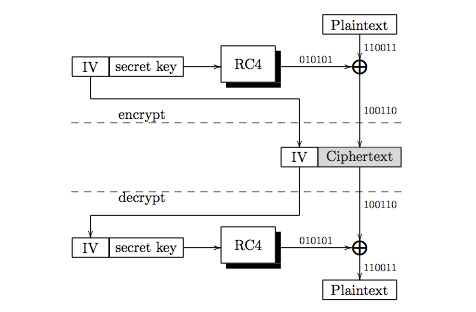
\includegraphics[keepaspectratio=true,width=0.5\linewidth]{WEP}  %skala och filnamn. 
  \caption{Översiktsbild WEP$^{\ref{RC4}}$} %figurtext.
  \end{center}
  \label{fig:overview}
\end{figure}
\newpage
Problemet med WEP är att den gemensamma nyckeln aldrig eller väldigt sällan byts ut eftersom metoden inte har stöd för att enheter byter krypteringsnyckel dynamiskt. Om samma nyckel används under lång tid kan angripare hitta mönster i paketen och således även nyckeln. Hur lång tid det tar att knäcka en WEP-nyckel beror på hur pass stor dataströmmen är, desto fler paket som skickas från noden till knytpunkten ju mer data med samma nyckel har avlyssnaren att arbeta med. På grund av bristerna i denna krypteringsmetod har en del andra utvecklats och kommit ut på marknaden under senare år.\footnote{\label{WEP}Kryptera mera. WEP, WPA och WPA2. http://www.omwlan.se/artiklar/kryptering-wep-wpa.aspx (hämtad 2014-04-10)}

\subsubsection{WPA}
Wifi Protected Access (WPA) skapades för att ersätta WEP och fylla igen dess säkerhetsbrister. WPA använder sig även den av chiffret RC4 men till skillnad från WEP har den en nyckel som dynamiskt genereras för varje enskilt paket. WPA finns i två versioner, Enterprise och Personal. De två olika versionerna har olika metoder för autentisering av noderna i nätverket. WPA-Personal även kallad Pre-Shared key, används av hemmaanvändare och här autentiserar varje nod med knytpunkten(routern) med en 256-bitars nyckel. WPA-Enterprise även kallad däremot 802.1x använder sig av en central server ofta kopplat till ett större nätverk (exempelvis på ett företag) som kontrollerar att certifikaten eller nycklarna är korrekta hos de noder som söker access. \footnote{\label{WPA}Wi-Fi Protected Access 2 (WPA2) Configuration Example. http://www.cisco.com/c/en/us/support/docs/wireless-mobility/wireless-lan-wlan/67134-wpa2-config.html (hämtad 2014-04-10)}
Förutom att WPA producerar nycklar dynamiskt har den även en rad andra tekniker som gör den säkrare än WEP. De krypterade paketen organiseras bättre och använder en vassare algoritm. WPA är säkrare än WEP men givetvis inte helt säkert. En ''hacker'' skulle t.ex. kunna använda en teknik som går ut på att skicka speciella paket till autentiseringsnoden och sedan studera hur dessa tas emot. Detta är dock betydligt svårare än WEP och den största risken med WPA är oftast att användare väljer ett allt för enkelt lösenord.$^{\ref{WEP}}$

\subsubsection{WPA2}
WPA2 är som det låter en vidareutveckling av WPA. Största föredelen med WPA var ju att den dynamiskt kunde byta ut nycklar, WPA2 gör nyckelskiftningen på ett mer elegant sätt. Den använder sig av Counter Mode Cipher Block Chaining Message Authentication Code Protocol eller helt enkelt CCMP. Detta krypterings protokoll har skapats utifrån svagheterna i WEP. Enkelt sagt kan man säga att protokollet gör så att avsändaren och mottagaren identifierar sig mot varandra och bestämmer en gemensam nyckel som i princip bara existerar vid ett tillfälle då ett enskilt paket skickas.$^{\ref{WPA}}$
\newpage

\subsection{Bluetooth}

Bluetooth är en global standard för trådlös kommunikation på korta avstånd och utvecklades av Ericsson 1994. Bluetooth utnyttjades till en början primärt som en ersättning för serielkommunikationskablar mellan enheter.\footnote{\label{BTweb}Bluetooth SIG. Fast Facts http://www.bluetooth.com/Pages/Fast-Facts.asp (Hämtad 2014-03-24)}
Bluetooth är fullt duplex och kan alltså skicka information i båda riktningar samtidigt. Dessutom kan Bluetooth sättas upp utan en tidigare existerande trådlös arkitektur och blir därför väldigt attraktiv för att para ihop enheter. Så som Bluetooth protokollet fungerar är det just parning mellan två enheter som är aktuellt. Bluetooth har fler aspekter som gör det särdeles bra för små mobila enheter.\footnote{\label{Gupta}Gupta, Naresh. Inside BLUETOOTH LOW ENERGY. Artech House, 2013}
\begin{itemize}
\item Låg strömförbrukning 
\item Låg kostnad
\item Liten formfaktor
\item Behöver ej fri sikt mellan enheterna
\end{itemize}

Bluetooth utnyttjar högfrekventa radiovågor mellan 2,4 GHz till 2,485 GHz för att sända information.$^{\ref{BTweb}}$

\subsubsection{Standarder för Bluetooth}
Hastighet för olika Bluetooth standarder:
\begin{itemize}
\item Bluetooth 1.2 - 1 Mbit/s 
\item Bluetooth 2.0 - 3 Mbit/s
\item Bluetooth 3.0 - 24 Mbit/s
\item Bluetooth 4.0 - 24 Mbit/s
\end{itemize}

Intressant att notera här är att Bluetooth 3.0 har en teoretisk överföringshastighet på 24 Mbit/s, men att denna överföring inte sker via Bluetooth, utan via den snabbare teknologin IEEE 802.11. 
Bluetooth 4.0 ökar inte hastigheten från 3.0 utan fokuserar istället på att spara in på strömförbrukning.$^{\ref{Gupta}}$


\subsubsection{Koppling av enheter}
En parkoppling mellan två Bluetooth-enheter, A och B, fungerar enligt principen att ena enheten, låt oss säga enhet B, måsta vara upptäckbar och måste alltså sända ut en form av identifikation, ofta i form av ett namn. Enhet A söker av vilka enheter den kan detektera och ger ofta en komplett lista till användaren över enheter som den detekterade. Nästa steg är att enhet A begär en koppling till enhet B. När kopplingen lyckas blir enhet A master och enhet B slave. Tvåvägskommunikation är nu möjlig mellan enheterna.\footnote{\label{Gupta2}Gupta, Naresh. 2013}

\subsubsection{Säkerhet}
Bluetooth är en förhållandevis säker kommunikationsform, men är självklart inte helt säker. En begränsning är att Bluetooth-enheterna ofta saknar inmatningsmöjligheter och display. Detta leder till att lösenord inte kan fyllas i eller ens genereras på enheterna. Om båda enheter har display och inmatningsmöjligheter kan en 16 siffror lång PIN-kod genereras som sedan måste fyllas i på den enhet som begär kopplingen. Detta skyddar mot de flesta former av avlyssning.
För enheter som saknar antingen display eller inmatningsmöjligheter finns andra möjliga lösningar. NFC, Near-Field Communication, kan användas för parning och då måste enheterna i princip röra varandra i parningsfasen men kan därefter utnyttja fulla räckvidden på Bluetooth. Detta kallas Out-of-Band Pairing.$^{\ref{Gupta2}}$

En annan typ av säkerhet som används är ''Just Work'', som utnyttjas när enheterna saknar både inmatningsmöjligheter och display. Ett exempel på detta är Bluetooth headsets till mobiltelefoner. Denna säkerhetsmetod kräver inte att användare utför någonting förutom själva kopplingen. Denna metod skyddar mot passiv avlyssning, men ej mot aktiv avlyssning. 
Aktiv avlyssning är när en enhet lägger sig mellan de två enheterna och vidarebefodrar kommunikationen mellan dem och kan vara väldigt svår att upptäcka.
Vid passiv avlyssning så försöker man endast lyssna av kommunikationen mellan två enheter.$^{\ref{Gupta2}}$

\subsubsection{RS232}
När den trådlösa delen av Bluetooth fungerar kan de vara intressant att diskutera vilken form av kommunikation själva hårdvaruenheterna som ska kommunicera med varandra får för typ av information. På en persondator, en vanlig mottagare av Bluetoothkommunikation, kommer den inbyggda Bluetooth mottagaren alternativt Bluetooth dongel att virtualiseras som en seriellport. Att kommunikationen blir seriell innebär att all information behöver konverteras till en följd av höga och låga bitar. RS232 är ett protokoll för sändning av just sådana paket. RS232 har stöd för asynkron kommunikation vilket blir eftertraktat när vi talar om trådlös kommunikation och information ofta kommer i små strömmer kontra en enda kontinuerlig ström. Vid programmering av mottagning och sändning via RS232 på en persondator finns oftast väl etablerade standardbibliotek att använda.
På enklare hårdvara t.ex. en ATmega1284p med ett FireFly BlueSMiRF GOLD modem, kommer man att variera spänningen på ett antal pinnar direkt för att styra diverse kommunikationssignaler samt för sändningen och mottagningen.
Protokollet specificerar upp hur många databitar och stoppbitar man har i varje paketström och vilken typ av paritetsbit som ska användas. Dessutom har den stöd för kommunikationssignaler som kan reglera flödet av information. Två vanliga signaler är CTS och RTS. CTS, Clear To Send, berättar för motparten att denna enhet är redo att ta emot data. RTS,Request To Send, ber om tillåtelse att skicka. Dataströmmen av ett paket kan ses övergripande i figur~\ref{fig:rs232}
En viktig sak att beakta vid asynkron kommunikation är att båda enheterna i förväg måste veta vilken hastighet som protokollet utnyttjar.\footnote{RS232 Data Interface, a Tutorial on Data Interface and cables. http://www.arcelect.com/rs232.htm, Hämtad (2014-04-10)}

\begin{figure}[htp]
  \begin{center}
  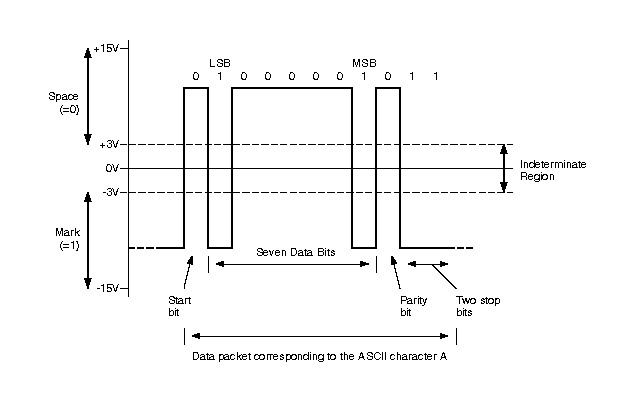
\includegraphics[keepaspectratio=true,width=0.5\linewidth]{RS232}  %skala och filnamn. 
  \caption{En RS232 sändning\label{fig:rs232}} %figurtext.
  \end{center}
\end{figure}


\subsection{Infrared (IR)}
IR kommunikation är en form av trådlös kommunikation där informationen skickas i form av IR-ljus och kräver därför direkt siktlinje mellan sändare och mottagare. En vanlig implementering av denna form av kommunikation är fjärrkontroller till TV-apparater.
Infrared Data Association Standards (IrDA) är en association bestående av ungefär 100 medlemsföretag. IrDA protokollen är ett såkallat Point-to-Point-protokoll och skickar alltså kommunikation mellan två enheter. IrDA har överföringshastighet på 2,4 kb/s upp till 4 Mb/s på upp till 1 meters avstånd. Vid länkning av två enheter kommer dessa alltid att kommunicera med 9,6 kb/s för att sedan komma överens om vilken hastighet som ska köras under dataöverföring.\footnote{\label{Carruthers}Carruthers, Jeffrey B. Wireless Infrared Communications,Department of Electrical and Computer Engineering
Boston University, 2002, http://iss.bu.edu/jbc/Publications/jbc-bc1.pdf (Hämtad 2014-03-24)}  
\newpage
\subsubsection{Långdistans IR kommunikation}
Flera hinder finns för konstruktion för långdistans kommunikation via IR. Dessa enheter behöver fri sikt och lider av signalstyrke förlust genom atmosfären. Vid byggnad till byggnad kommunikation med IR får man även problemet med att byggnader svajar något vilket kan leda till att direkt länken bryts.\footnote{\label{Carruthers2}Carruthers, Jeffrey B. W 2002}

\subsubsection{Säkerhet}
Säkerhet i IR-kommunikationsfallet vid kortdistans, handlar mer eller mindre om det faktum att avstånden för överföring är såpass små att hackningförsök blir inaktuella, men kryptering av data på mottagar- och sändarsida är självklart möjligt.$^{\ref{Carruthers2}}$

\subsection{ZigBee}
ZigBee är en standard för trådlös styrning och övervakning som används i hem och industrier men även i andra övervaknings- och styrningsapplikationer där låg strömförbrukning och hög tillgänglighet är i fokus. Zigbee-standarden erbjuder näverks-, säkerhets- och applikationssupport ovanpå IEEE 802.15.4 standarden. Plattformen har stöd för stjärnnät och trädstruktur men mesh-arkitektur är mest populär.

\subsubsection{IEEE 802.15}
Standarden definierar protokoll och sammankoppling av enheter i ett wireless personal area network (WPAN). IEEE 802.15.4 (LR-WPAN) som ZigBee använder sig av är en undergrupp till denna standard och har egenskaper som låg datahastighet men med lång batteritid. Datahastigheten kommer maximalt att kunna uppnå 250 kb/s men räcker gott och väl till dess användningsområde. Det kan också skalas ner till 20 kb/s för att kunna hantera sensorer och dylikt.\footnote{\label{IEEE} Part 15.4 Wireless Medium Access Control (MAC) and Physical Layer (PHY) Specifications for Low-Rate Wireless Personal Area Networks (LR-WPANs). The Institute of Electrical and Electronics Engineers, Inc. (2003)}


Standarden definierar det fysiska lagret samt datalänklagret i OSI-modellen.\footnote{Zimmermann, Hubert (April 1980). OSI Reference Model — The ISO Model of Architecture for Open Systems Interconnection. IEEE Transactions on Communications 28 (4): 425–432. doi:10.1109/TCOM.1980.1094702} 


\subsubsection{Mesh-arkitektur}
Mesh-arkitekturen är en nätstruktur där alla noder i nätet har kontakt med minst 2 noder samtidigt. Detta ger i sin tur hög redundans vilket leder till högre säkerhet på kommunikationen. Strukturen är således tillförlitlig och erbjuder bra skydd mot varianser i signalstyrka som kan skapas av interferens eller multipla signaler.\footnote{\label{eltidning} Wheeler, Andy. Krama saften ur Zigbee. Elektronik Tidningen (2005).(Hämtad 2014-03-24)}

\subsubsection{Säkerhet}
Säkerhetsåtgärderna i denna standard är baserade på symmetrisk kryptering även kallad delad-nyckel-kryptering. Denna metod använder samma nyckel vid kryptering som vid dekryptering och detta innebär givetvis en svaghet i säkerheten, men en tillräckligt stor nyckel ger oftast fullt tillräcklig säkerhet. 
Standarden använder sig även av kontroll av vilka noder som är tillåtna, alltså vilka som får skicka data. Varje nod har en access control list (ACL), en lista över noder som är godkända att kommunicera med som noden har för att kunna jämföra med inkommande förfrågningar från andra noder.\footnote{Zimmermann, Hubert 1980} 
Med ZigBee följer även ett koncept som heter ''Trust Center'' som möjliggör för noder att ansluta till nätverket, distribuera nycklar och ge möjligheten att kontrollera säkerheten hela vägen mellan två enheter. Det finns två olika säkerhetsnivåer, en gjord för hemmabruk och en för kommersiella applikationer. Den största skillnaden mellan de båda nivåerna är att den sistnämnda skapar och underhåller säkerhetsnycklar.\footnote{Wheeler Andy 2005}

\newpage

\section{Resultat}
WLAN är en fantastisk teknik för skapandet av nätverk mellan flera enheter och har fördelen att ha stöd för uppkoppling och delning av internet via routrar. WLAN har dessutom lång räckvidd, stark säkerhet och hög överföringshastighet.
  
Bluetooth skapar solida kopplingar mellan enskilda enheter och har förhållandevis enkelt programmeringsinterface både för högnivåspråk och lågnivåspråk. Dessutom har Bluetooth en relativt hög överföringshastighet. Det som lämnar lite att önska hos Bluetooth är säkerheten hos enklare och äldre enheter.

IRkommunikation har kort räckvidd och kräver väldig stabilitet hos både mottagare och sändare. Om synsikten mellan sändare och mottagare bryts kommer även kommunikationen att brytas. Hastigheten hos IR är relativt hög. 

ZigBee kan beskrivas som en enklare version av Bluetooth och har inga egentliga fördelar över bluetooth. 

\section{Diskussion}
Utifrån fördjupningen kan vi sluta oss till att IR-kommunikation inte är ett alternativ för ett mobilt robotfordon. IR kräver antingen relativt stillastående föremål eller korta avstånd. Dessutom krävs sändar-mottagarstruktur på båda sidor då ett mobilt robotfordon rimligen ska kunna både skicka och ta emot data.
IEEE802.11 är ett starkt alternativ tack vare sin höga överföringshastighet och långa räckvidd, men en oro är störningar som kan uppstå då många signaler populerar IEEE802.11 bandet, samt att en existerande nätverksstruktur behövs användas.
Bluetooth och IEEE802.11 klarar båda två kommunikation i båda riktningar, har tillräcklig säkerhet och stabilitet. Bluetooths användarvänlighet och det faktum att den är Point-to-Point får avgöra i detta fall och bluetooth blir rekommendationen vi lämnar på kommunikationen med autonomt robotfordon.

\newpage 
\section*{Referenser}

Bluetooth SIG. Fast Facts http://www.bluetooth.com/Pages/Fast-Facts.asp (Hämtad 2014-03-24)

Chaabouni, Rafik. Break WEP Faster with Statistical Analysis, Institute of Technology Lausanne, 2006. http://lasecwww.epfl.ch/pub/lasec/doc/cha06.pdf (hämtad 2014-04-10)

Kryptera mera. WEP, WPA och WPA2. http://www.omwlan.se/artiklar/kryptering-wep-wpa.aspx (hämtad 2014-04-10)

Gupta, Naresh. \emph{Inside BLUETOOTH LOW ENERGY.} Artech House, 2013

Holger Karl, Andreas Willig. \emph{Protocols and Architectures for Wireless Sensor Networks}, Wiley, 2005

Lopez-Aguilera, Elena. \emph{Study on the influence of transmission errors on RSNA authentication mechanisms in IEEE 802.11 WLAN.}, Computer Communications Volume: 41 Issue: 5 (2014-01-01) p. 76-93

Part 15.4 Wireless Medium Access Control (MAC) and Physical Layer (PHY) Specifications for Low-Rate Wireless Personal Area Networks (LR\text{-}WPANs). The Institute of Electrical and Electronics Engineers, Inc. (2003) \\ http://www.engineering.uiowa.edu/~mcover/lab4/802.15.4-2003.pdf (Hämtad 2014-03-24)

Wheeler, Andy. Krama saften ur Zigbee. \emph{Elektronik Tidningen (2005).} \\ http://etn.se/index.php?option=com\_content\&task=view\&id=18463\&Itemid=66 (Hämtad 2014-03-24)

Zimmermann, Hubert (April 1980).\emph{ OSI Reference Model — The ISO Model of Architecture for Open Systems Interconnection.} IEEE Transactions on Communications 28 (4): 425–432. doi:10.1109/TCOM.1980.1094702


\end{document}